\part{Preparação da pesquisa}

% ----------------------------------------------------------
% Este capítulo, utilizado por diferentes exemplos do abnTeX2, ilustra o uso de
% comandos do abnTeX2 e de LaTeX.
% ----------------------------------------------------------

\chapter{Resultados de comandos}\label{cap_exemplos}

\chapterprecis{Isto é uma sinopse de capítulo. A ABNT não traz nenhuma
normatização a respeito desse tipo de resumo, que é mais comum em romances 
e livros técnicos.}\index{sinopse de capítulo}

% ---
\section{Codificação dos arquivos: UTF8}
% ---

A codificação de todos os arquivos do \abnTeX\ é \texttt{UTF8}. É necessário que
você utilize a mesma codificação nos documentos que escrever, inclusive nos
arquivos de base bibliográficas |.bib|.

% ---
\section{Citações diretas}
\label{sec-citacao}
% ---

\index{citações!diretas}Utilize o ambiente \texttt{citacao} para incluir
citações diretas com mais de três linhas:

\begin{citacao}
As citações diretas, no texto, com mais de três linhas, devem ser
destacadas com recuo de 4 cm da margem esquerda, com letra menor que a do texto
utilizado e sem as aspas. No caso de documentos datilografados, deve-se
observar apenas o recuo \cite[5.3]{NBR10520:2002}.
\end{citacao}

Use o ambiente assim:
\begin{verbatim}
\begin{citacao}
As citações diretas, no texto, com mais de três linhas [...] deve-se
observar apenas o recuo \cite[5.3]{NBR10520:2002}.
\end{citacao}
\end{verbatim}

O ambiente \texttt{citacao} pode receber como parâmetro opcional um nome de
idioma previamente carregado nas opções da classe (\autoref{sec-hifenizacao}). Nesse
caso, o texto da citação é automaticamente escrito em itálico e a hifenização é
ajustada para o idioma selecionado na opção do ambiente. Por exemplo:
\begin{verbatim}
\begin{citacao}[english]
Text in English language in italic with correct hyphenation.
\end{citacao}
\end{verbatim}

Tem como resultado:
\begin{citacao}[english]
Text in English language in italic with correct hyphenation.
\end{citacao}

\index{citações!simples}Citações simples, com até três linhas, devem ser
incluídas com aspas. Observe que em \LaTeX\ as aspas iniciais são diferentes das
finais: ``Amor é fogo que arde sem se ver''.

% ---
\section{Notas de rodapé}
% ---

As notas de rodapé são detalhadas pela NBR 14724:2011 na seção 5.2.1\footnote{As
notas devem ser digitadas ou datilografadas dentro das margens, ficando
separadas do texto por um espaço simples de entre as linhas e por filete de 5
cm, a partir da margem esquerda. Devem ser alinhadas, a partir da segunda linha
da mesma nota, abaixo da primeira letra da primeira palavra, de forma a destacar
o expoente, sem espaço entre elas e com fonte menor
\citeonline[5.2.1]{NBR14724:2011}.}\footnote{Caso uma série de notas sejam
criadas sequencialmente, o \abnTeX\ instrui o \LaTeX\ para que uma vírgula seja
colocada após cada número do expoente que indica a nota de rodapé no corpo do
texto.}\footnote{Verifique se os números do expoente possuem uma vírgula para
dividi-los no corpo do texto.}. 


% ---
\section{Tabelas}
% ---

\index{tabelas}A \autoref{tab-nivinv} é um exemplo de tabela construída em \LaTeX.
\begin{table}[htb]
\ABNTEXfontereduzida
\caption[Níveis de investigação]{Níveis de investigação.}
\label{tab-nivinv}
\begin{tabular}{p{2.6cm}|p{6.0cm}|p{2.25cm}|p{3.40cm}}
  %\hline
   \textbf{Nível de Investigação} & \textbf{Insumos}  & \textbf{Sistemas de Investigação}  & \textbf{Produtos}  \\
    \hline
    Meta-nível & Filosofia\index{filosofia} da Ciência  & Epistemologia &
    Paradigma  \\
    \hline
    Nível do objeto & Paradigmas do metanível e evidências do nível inferior &
    Ciência  & Teorias e modelos \\
    \hline
    Nível inferior & Modelos e métodos do nível do objeto e problemas do nível inferior & Prática & Solução de problemas  \\
   % \hline
\end{tabular}
\legend{Fonte: \citeonline{van86}}
\end{table}

Já a \autoref{tabela-ibge} apresenta uma tabela criada conforme o padrão do
\citeonline{ibge1993} requerido pelas normas da ABNT para documentos técnicos e
acadêmicos.
\begin{table}[htb]
\IBGEtab{%
  \caption{Um Exemplo de tabela alinhada que pode ser longa
  ou curta, conforme padrão IBGE.}%
  \label{tabela-ibge}
}{%
  \begin{tabular}{ccc}
  \toprule
   Nome & Nascimento & Documento \\
  \midrule \midrule
   Maria da Silva & 11/11/1111 & 111.111.111-11 \\
  \midrule 
   João Souza & 11/11/2111 & 211.111.111-11 \\
  \midrule 
   Laura Vicuña & 05/04/1891 & 3111.111.111-11 \\
  \bottomrule
\end{tabular}%
}{%
  \fonte{Produzido pelos autores.}%
  \nota{Esta é uma nota, que diz que os dados são baseados na
  regressão linear.}%
  \nota[Anotações]{Uma anotação adicional, que pode ser seguida de várias
  outras.}%
  }
\end{table}


% ---
\section{Figuras}
% ---

\index{figuras}Figuras podem ser criadas diretamente em \LaTeX,
como o exemplo da \autoref{fig_circulo}.
\begin{figure}[htb]
	\caption{\label{fig_circulo}A delimitação do espaço}
	\begin{center}
	    \setlength{\unitlength}{5cm}
		\begin{picture}(1,1)
		\put(0,0){\line(0,1){1}}
		\put(0,0){\line(1,0){1}}
		\put(0,0){\line(1,1){1}}
		\put(0,0){\line(1,2){.5}}
		\put(0,0){\line(1,3){.3333}}
		\put(0,0){\line(1,4){.25}}
		\put(0,0){\line(1,5){.2}}
		\put(0,0){\line(1,6){.1667}}
		\put(0,0){\line(2,1){1}}
		\put(0,0){\line(2,3){.6667}}
		\put(0,0){\line(2,5){.4}}
		\put(0,0){\line(3,1){1}}
		\put(0,0){\line(3,2){1}}
		\put(0,0){\line(3,4){.75}}
		\put(0,0){\line(3,5){.6}}
		\put(0,0){\line(4,1){1}}
		\put(0,0){\line(4,3){1}}
		\put(0,0){\line(4,5){.8}}
		\put(0,0){\line(5,1){1}}
		\put(0,0){\line(5,2){1}}
		\put(0,0){\line(5,3){1}}
		\put(0,0){\line(5,4){1}}
		\put(0,0){\line(5,6){.8333}}
		\put(0,0){\line(6,1){1}}
		\put(0,0){\line(6,5){1}}
		\end{picture}
	\end{center}
	\legend{Fonte: os autores}
\end{figure}

As figuras podem, ainda, ser incorporadas de arquivos externos, como é o caso da
\autoref{fig_grafico}. Se a figura a ser incluída se tratar de um diagrama, um
gráfico ou uma ilustração que você mesmo produza, priorize o uso de imagens
vetoriais no formato PDF. Com isso, o tamanho do arquivo final do trabalho será
menor, e as imagens terão uma apresentação melhor, principalmente quando
impressas, uma vez que imagens vetorias são perfeitamente escaláveis para
qualquer dimensão. Nesse caso, se for utilizar o Microsoft Excel para produzir
gráficos, ou o Microsoft Word para produzir ilustrações, exporte-os como PDF e
os incorpore ao documento conforme o exemplo abaixo. No entanto, para manter a
coerência no uso de software livre (já que você está usando \LaTeX e \abnTeX),
teste a ferramenta \textsf{InkScape}\index{InkScape}
(\url{http://inkscape.org/}). Ela é uma excelente opção de código-livre para
produzir ilustrações vetoriais, similar ao CorelDraw\index{CorelDraw} ou ao Adobe
Illustrator\index{Adobe Illustrator}. De todo modo, caso não seja possível
utilizar arquivos de imagens como PDF, utilize qualquer outro formato, como
JPEG, GIF, BMP, etc. Nesse caso, você pode tentar aprimorar as imagens
incorporadas com o software livre \textsf{Gimp}\index{Gimp}
(\url{http://www.gimp.org/}). Ele é uma alternativa livre ao Adobe
Photoshop\index{Adobe Photoshop}.
\begin{figure}[htb]
	\caption{\label{fig_grafico}Gráfico produzido em Excel e salvo como PDF}
	\begin{center}
	    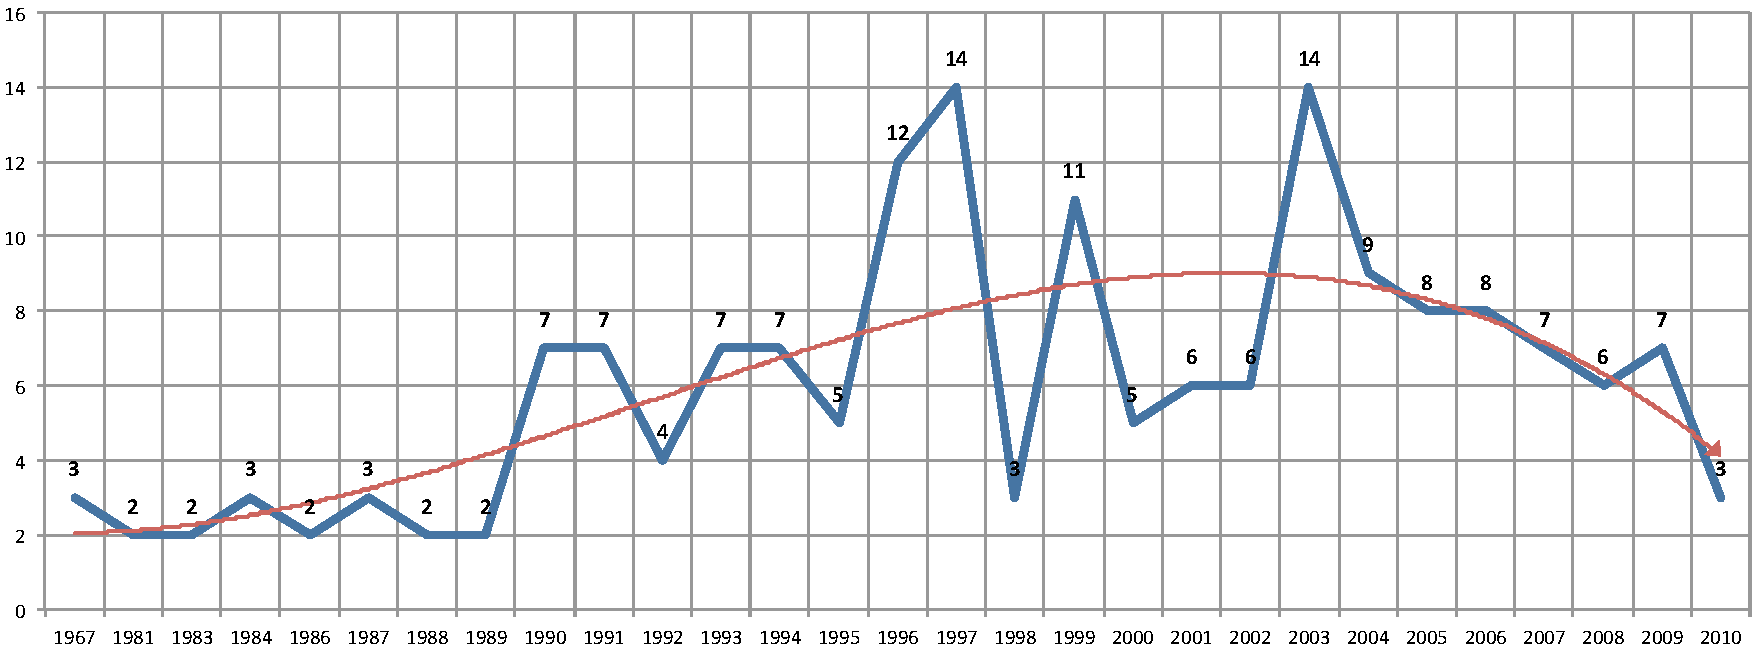
\includegraphics[scale=0.5]{abntex2-modelo-img-grafico.pdf}
	\end{center}
	\legend{Fonte: \citeonline[p. 24]{araujo2012}}
\end{figure}

% ---
\subsection{Figuras em \emph{minipages}}
% ---

\emph{Minipages} são usadas para inserir textos ou outros elementos em quadros
com tamanhos e posições controladas. Veja o exemplo da
\autoref{fig_minipage_imagem1} e da \autoref{fig_minipage_grafico2}.
\begin{figure}[htb]
 \label{teste}
 \centering
  \begin{minipage}{0.45\textwidth}
    \centering
    \caption{Imagem 1 da minipage} \label{fig_minipage_imagem1}
    
\includegraphics[scale=0.8]{abntex2-modelo-img-marca.pdf}
    \legend{Fonte: Produzido pelos autores}
  \end{minipage}
  \hfill
  \begin{minipage}{0.45\textwidth}
    \centering
    \caption{Grafico 2 da minipage} \label{fig_minipage_grafico2}
    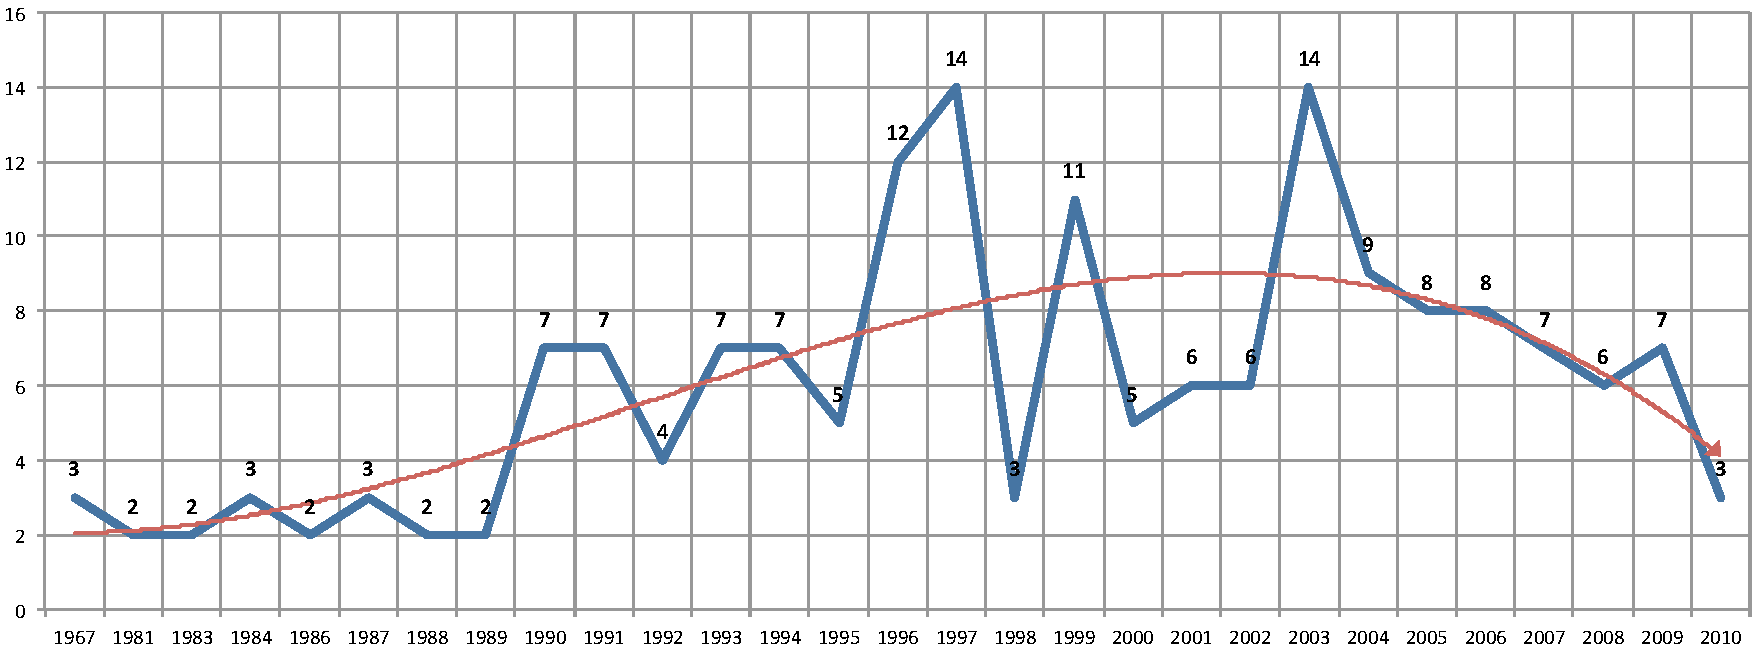
\includegraphics[scale=0.2]{abntex2-modelo-img-grafico.pdf}
    \legend{Fonte: \citeonline[p. 24]{araujo2012}}
  \end{minipage}
\end{figure}

Observe que, segundo a \citeonline[seções 4.2.1.10 e 5.8]{NBR14724:2011}, as
ilustrações devem sempre ter numeração contínua e única em todo o documento:
\begin{citacao}
Qualquer que seja o tipo de ilustração, sua identificação aparece na parte
superior, precedida da palavra designativa (desenho, esquema, fluxograma,
fotografia, gráfico, mapa, organograma, planta, quadro, retrato, figura,
imagem, entre outros), seguida de seu número de ordem de ocorrência no texto,
em algarismos arábicos, travessão e do respectivo título. Após a ilustração, na
parte inferior, indicar a fonte consultada (elemento obrigatório, mesmo que
seja produção do próprio autor), legenda, notas e outras informações
necessárias à sua compreensão (se houver). A ilustração deve ser citada no
texto e inserida o mais próximo possível do trecho a que se
refere. \cite[seção 5.8]{NBR14724:2011}
\end{citacao}

% ---
\section{Subfiguras}
% ---

Como pode ser visto em \citeonline[seção 5.8]{NBR14724:2011}, as subfiguras não 
são elementos regulamentados pelas normas ABNT. A classe \textsf{memoir} dispõe
de comandos para inserção e manejo de subfiguras sem a necessidade de adição de
novos pacotes. Como exemplo, podemos dispor de subfiguras tais como as que seguem
na \autoref{fig_subfigs}, respectivamente as subfiguras \ref{subfig_one} e 
\ref{subfig_two}, juntamente com a \autoref{subfig_three}.
\begin{figure}
  \centering
  \caption{Usando subfiguras}
  \label{fig_subfigs}
  \subtop[\label{subfig_one}Primeira subfigura]{%
    \includegraphics[width=0.3\linewidth]{example-image-a}}
  \subtop[\label{subfig_two}Segunda subfigura]{%
    \includegraphics[width=0.3\linewidth]{example-image-b}}
  \subtop[queisso][\label{subfig_three}Terceira subfigura, com título em mais de uma linha]{%
    \includegraphics[width=0.3\linewidth]{example-image-c}}
  \legend{Fonte: Extraído de \TeX--\LaTeX\ Stack Exchange}
\end{figure}

% ---
\section{Expressões matemáticas}
\label{math-expr}
% ---

\index{expressões matemáticas}Use o ambiente \texttt{equation} para escrever
expressões matemáticas numeradas:
\begin{equation}
  \forall x \in X, \quad \exists \: y \leq \epsilon
\end{equation}

Escreva expressões matemáticas entre \$ e \$, como em $ \lim_{x \to \infty}
\exp(-x) = 0 $, para que fiquem na mesma linha.

Também é possível usar colchetes para indicar o início de uma expressão
matemática que não é numerada.
\[
\left|\sum_{i=1}^n a_ib_i\right|
\le
\left(\sum_{i=1}^n a_i^2\right)^{1/2}
\left(\sum_{i=1}^n b_i^2\right)^{1/2}
\]

Consulte mais informações sobre expressões matemáticas em
\url{https://github.com/abntex/abntex2/wiki/Referencias}.

%---
\section{Teoremas, lemas, proposições e outros ambientes}
% ---

A comunidade matemática utiliza com bastante frequência os ambientes 
\textsf{teorema}, \textsf{lema}, \textsf{proposição} e outros ambientes 
relacionados. Tais definições não necessitam de pacotes adicionais e
podem ser realizadas nas configurações globais.

\begin{definition}[Limite]
  \label{definicao}
  Sejam $f\colon A\rightarrow\mathds{R}$ uma função e $b\in\mathds{R}$ tais 
  que para todo intervalo aberto $I$, contendo $b$, tem-se 
  $I\cap(A-\{b\})\neq\emptyset$. O número real $L$ é o limite de $f(x)$ quando
  $x$ aproxima-se de $b$ quando para todo número $\epsilon>0$, existe $\delta>0$
  ($\delta$ dependendo de $\epsilon$), tal que, se $x\in A$ e $0<|x-b|<\delta$
  então $|f(x)-L|<\epsilon$.
\end{definition}

\begin{proposition}[Unicidade do limnite]
  \label{proposicao}
  Se $\lim_{x\rightarrow b}f(x)=L_1$ e $\lim_{x\rightarrow b}f(x)=L_2$
  ($L_1,L_2\in\mathds{R}$), então $L_1=L_2$.
\end{proposition}

\begin{corollary}
  \label{corolario}
  Se as funções $f(x)$ e $g(x)$ são tais que $f(x) = g(x)$ exceto num ponto $b$,
  então $\lim_{x\rightarrow b}f(x)=\lim_{x\rightarrow b}g(x)$, desde que exista
  um dos limites.
\end{corollary}

\begin{lemma}
  \label{lema}
  Se $a|b$ então $\mathrm{mdc}(a,b)=a$.
\end{lemma}

\begin{theorem}[do Ponto Fixo de Brouwer]
  \label{teorema}
  Se $f\colon[0,1]\rightarrow[0,1]$ é contínua, então $f$ tem ponto fixo.
\end{theorem}
\begin{proof}
  Este ambiente só está definido para o pacote \textsf{amsthm}.
\end{proof}


\begin{conjecture}[de Poincaré]
  \label{conjectura}
  Toda variedade fechada simplesmente conexa de dimensão 3 é equivalente à esfera
  3-dimensional.
\end{conjecture}

% \begin{notation}
%   \label{notacao}
%   oioioi
% \end{notation}

\begin{remark}
  \label{observacao}
  Os gráficos de $f(x) + c$, $f(x + c)$, $cf(x)$ e $f(c x)$ ($c\in\mathds{R}$) 
  podem ser obtidos diretamente do gráfico de $f(x)$.
\end{remark}

% \begin{note}
%   \label{nota}
%   oioioi
% \end{note}

\begin{example}
  \label{exemplo}
  A composta de funções afins é uma função afim.\newline De fato, sejam $f(x)=m_1x+b_1$ e
  $g(x)=m_2x+b_2$. Então, $(g\circ f)(x)=(m_1m_2)x+m_2b_1+b_2$ e 
  $(f\circ g)(x)=(m_1m_2)x+m_1b_2+b_1$.
\end{example}

Para citar no texto, basta usar \textsf{label} dentro de cada ambiente desejado:
\autoref{definicao}, \autoref{proposicao}, \autoref{corolario}, \autoref{lema},
\autoref{teorema}, \autoref{conjectura}, \autoref{observacao}, \autoref{exemplo}.
%, \autoref{}, \autoref{}.

% ---
\section{Enumerações: alíneas e subalíneas}
% ---

\index{alíneas}\index{subalíneas}\index{incisos}Quando for necessário enumerar
os diversos assuntos de uma seção que não possua título, esta deve ser
subdividida em alíneas \cite[4.2]{NBR6024:2012}:
\begin{alineas}
  \item os diversos assuntos que não possuam título próprio, dentro de uma mesma
  seção, devem ser subdivididos em alíneas; 
  
  \item o texto que antecede as alíneas termina em dois pontos;
  \item as alíneas devem ser indicadas alfabeticamente, em letra minúscula,
  seguida de parêntese. Utilizam-se letras dobradas, quando esgotadas as
  letras do alfabeto;

  \item as letras indicativas das alíneas devem apresentar recuo em relação à
  margem esquerda;

  \item o texto da alínea deve começar por letra minúscula e terminar em
  ponto-e-vírgula, exceto a última alínea que termina em ponto final;

  \item o texto da alínea deve terminar em dois pontos, se houver subalínea;

  \item a segunda e as seguintes linhas do texto da alínea começa sob a
  primeira letra do texto da própria alínea;
  
  \item subalíneas \cite[4.3]{NBR6024:2012} devem ser conforme as alíneas a
  seguir:

  \begin{alineas}
     \item as subalíneas devem começar por travessão seguido de espaço;

     \item as subalíneas devem apresentar recuo em relação à alínea;

     \item o texto da subalínea deve começar por letra minúscula e terminar em
     ponto-e-vírgula. A última subalínea deve terminar em ponto final, se não
     houver alínea subsequente;

     \item a segunda e as seguintes linhas do texto da subalínea começam sob a
     primeira letra do texto da própria subalínea.
  \end{alineas}
  
  \item no \abnTeX\ estão disponíveis os ambientes \texttt{incisos} e
  \texttt{subalineas}, que em suma são o mesmo que se criar outro nível de
  \texttt{alineas}, como nos exemplos à seguir:
  
  \begin{incisos}
    \item \textit{Um novo inciso em itálico};
  \end{incisos}
  
  \item Alínea em \textbf{negrito}:
  
  \begin{subalineas}
    \item \textit{Uma subalínea em itálico};
    \item \underline{\textit{Uma subalínea em itálico e sublinhado}}; 
  \end{subalineas}
  
  \item Última alínea com \emph{ênfase}.
  
\end{alineas}

% ---
\section{Espaçamento entre parágrafos e linhas}
% ---

\index{espaçamento!dos parágrafos}O tamanho do parágrafo, espaço entre a margem
e o início da frase do parágrafo, é definido por:
\begin{verbatim}
   \setlength{\parindent}{2.0cm}
\end{verbatim}

\index{espaçamento!do primeiro parágrafo}Por padrão, não há espaçamento no
primeiro parágrafo de cada início de divisão do documento
(\autoref{sec-divisoes}). Porém, você pode definir que o primeiro parágrafo
também seja indentado, como é o caso deste documento. Para isso, apenas inclua o
pacote \textsf{indentfirst} no preâmbulo do documento:
\begin{verbatim}
 \usepackage{indentfirst}    % Indenta o primeiro parágrafo de cada seção.
\end{verbatim}

\index{espaçamento!entre os parágrafos}O espaçamento entre um parágrafo e outro
pode ser controlado por meio do comando:
\begin{verbatim}
  \setlength{\parskip}{0.2cm}  % tente também \onelineskip
\end{verbatim}

\index{espaçamento!entre as linhas}O controle do espaçamento entre linhas é
definido por:
\begin{verbatim}
  \OnehalfSpacing       % espaçamento um e meio (padrão); 
  \DoubleSpacing        % espaçamento duplo
  \SingleSpacing        % espaçamento simples	
\end{verbatim}

Para isso, também estão disponíveis os ambientes:
\begin{verbatim}
  \begin{SingleSpace} ...\end{SingleSpace}
  \begin{Spacing}{hfactori} ... \end{Spacing}
  \begin{OnehalfSpace} ... \end{OnehalfSpace}
  \begin{OnehalfSpace*} ... \end{OnehalfSpace*}
  \begin{DoubleSpace} ... \end{DoubleSpace}
  \begin{DoubleSpace*} ... \end{DoubleSpace*} 
\end{verbatim}

Para mais informações, consulte \citeonline[p. 47-52 e 135]{memoir}.

% ---
\section{Inclusão de outros arquivos}\label{sec-include}
% ---

É uma boa prática dividir o seu documento em diversos arquivos, e não
apenas escrever tudo em um único. Esse recurso foi utilizado neste
documento. Para incluir diferentes arquivos em um arquivo principal,
de modo que cada arquivo incluído fique em uma página diferente, utilize o
comando:
\begin{verbatim}
   \include{documento-a-ser-incluido}      % sem a extensão .tex
\end{verbatim}

Para incluir documentos sem quebra de páginas, utilize:
\begin{verbatim}
   \input{documento-a-ser-incluido}      % sem a extensão .tex
\end{verbatim}

% ---
\section{Compilar o documento \LaTeX}
% ---

Geralmente os editores \LaTeX, como o
TeXlipse\footnote{\url{http://texlipse.sourceforge.net/}}, o
Texmaker\footnote{\url{http://www.xm1math.net/texmaker/}}, entre outros,
compilam os documentos automaticamente, de modo que você não precisa se
preocupar com isso.

No entanto, você pode compilar os documentos \LaTeX usando os seguintes
comandos, que devem ser digitados no \emph{Prompt de Comandos} do Windows ou no
\emph{Terminal} do Mac ou do Linux:
\begin{verbatim}
  pdflatex ARQUIVO_PRINCIPAL.tex
  bibtex ARQUIVO_PRINCIPAL.aux
  makeindex ARQUIVO_PRINCIPAL.idx 
  makeindex ARQUIVO_PRINCIPAL.nlo -s nomencl.ist -o ARQUIVO_PRINCIPAL.nls
  pdflatex ARQUIVO_PRINCIPAL.tex
  pdflatex ARQUIVO_PRINCIPAL.tex
\end{verbatim}

% ---
\section{Remissões internas}
% ---

Ao nomear a \autoref{tab-nivinv} e a \autoref{fig_circulo}, apresentamos
um exemplo de remissão interna que também pode ser feita quando indicamos
o \autoref{cap_exemplos}, que tem o nome \emph{\nameref{cap_exemplos}}.
O número do capítulo indicado é \ref{cap_exemplos}, que se inicia à
\autopageref{cap_exemplos}\footnote{O número da página de uma remissão
pode ser obtida também assim:
\pageref{cap_exemplos}.}.
Veja a \autoref{sec-divisoes} para outros exemplos de remissões internas
entre seções, subseções e subsubseções.

O código usado para produzir o texto desta seção é:
\begin{verbatim}
Ao nomear a \autoref{tab-nivinv} e a \autoref{fig_circulo}, apresentamos
um exemplo de remissão interna que também pode ser feita quando indicamos
o \autoref{cap_exemplos}, que tem o nome \emph{\nameref{cap_exemplos}}.
O número do capítulo indicado é \ref{cap_exemplos}, que se inicia à
\autopageref{cap_exemplos}\footnote{O número da página de uma remissão
pode ser obtida também assim:
\pageref{cap_exemplos}.}.
Veja a \autoref{sec-divisoes} para outros exemplos de remissões internas
entre seções, subseções e subsubseções.
\end{verbatim}

% ---
\section{Divisões do documento: seção}\label{sec-divisoes}
% ---

Esta seção testa o uso de divisões de documentos. Esta é a
\autoref{sec-divisoes}. Veja a \autoref{sec-divisoes-subsection}.

\subsection{Divisões do documento: subseção}\label{sec-divisoes-subsection}

Isto é uma subseção. Veja a \autoref{sec-divisoes-subsubsection}, que é uma
\texttt{subsubsection} do \LaTeX, mas é impressa chamada de ``subseção'' porque
no Português não temos a palavra ``subsubseção''.

\subsubsection{Divisões do documento: subsubseção}
\label{sec-divisoes-subsubsection}

Isto é uma subsubseção.

\subsubsection{Divisões do documento: subsubseção}

Isto é outra subsubseção.

\subsection{Divisões do documento: subseção}\label{sec-exemplo-subsec}

Isto é uma subseção.

\subsubsection{Divisões do documento: subsubseção}

Isto é mais uma subsubseção da \autoref{sec-exemplo-subsec}.


\subsubsubsection{Esta é uma subseção de quinto
nível}\label{sec-exemplo-subsubsubsection}

Esta é uma seção de quinto nível. Ela é produzida com o seguinte comando:
\begin{verbatim}
\subsubsubsection{Esta é uma subseção de quinto
nível}\label{sec-exemplo-subsubsubsection}
\end{verbatim}

\subsubsubsection{Esta é outra subseção de quinto nível}\label{sec-exemplo-subsubsubsection-outro}

Esta é outra seção de quinto nível.


\paragraph{Este é um parágrafo numerado}\label{sec-exemplo-paragrafo}

Este é um exemplo de parágrafo nomeado. Ele é produzida com o comando de
parágrafo:
\begin{verbatim}
\paragraph{Este é um parágrafo nomeado}\label{sec-exemplo-paragrafo}
\end{verbatim}

A numeração entre parágrafos numeradaos e subsubsubseções são contínuas.

\paragraph{Esta é outro parágrafo numerado}\label{sec-exemplo-paragrafo-outro}

Esta é outro parágrafo nomeado.

% ---
\section{Este é um exemplo de nome de seção longo. Ele deve estar
alinhado à esquerda e a segunda e demais linhas devem iniciar logo abaixo da
primeira palavra da primeira linha}
% ---

Isso atende à norma \citeonline[seções de 5.2.2 a 5.2.4]{NBR14724:2011} 
 e \citeonline[seções de 3.1 a 3.8]{NBR6024:2012}.

% ---
\section{Diferentes idiomas e hifenizações}
\label{sec-hifenizacao}
% ---

Para usar hifenizações de diferentes idiomas, inclua nas opções do documento o
nome dos idiomas que o seu texto contém. Por exemplo (para melhor
visualização, as opções foram quebras em diferentes linhas):
\begin{verbatim}
\documentclass[
	12pt,
	openright,
	twoside,
	a4paper,
	english,
	spanish,
	brazil
	]{abntex2}
\end{verbatim}

O idioma português-brasileiro (\texttt{brazil}) é incluído automaticamente pela
classe \textsf{abntex2}. Porém, mesmo assim a opção \texttt{brazil} deve ser
informada como a última opção da classe para que todos os pacotes reconheçam o
idioma. Vale ressaltar que a última opção de idioma é a utilizada por padrão no
documento. Desse modo, caso deseje escrever um texto em inglês que tenha
citações em português e em espanhol, você deveria usar o preâmbulo como abaixo:
\begin{verbatim}
\documentclass[
	12pt,
	openright,
	twoside,
	a4paper,
	spanish,
	brazil,
	english
	]{abntex2}
\end{verbatim}

A lista completa de idiomas suportados, bem como outras opções de hifenização,
estão disponíveis em \citeonline[p.~5-6]{babel}.

Exemplo de hifenização em inglês\footnote{Extraído de:
\url{http://en.wikibooks.org/wiki/LaTeX/Internationalization}}:

\begin{otherlanguage*}{english}
\textit{Text in English language. This environment switches all language-related
definitions, like the language specific names for figures, tables etc. to the other
language. The starred version of this environment typesets the main text
according to the rules of the other language, but keeps the language specific
string for ancillary things like figures, in the main language of the document.
The environment hyphenrules switches only the hyphenation patterns used; it can
also be used to disallow hyphenation by using the language name
`nohyphenation'.}
\end{otherlanguage*}

% Pequeno texto em espanhol\footnote{Extraído de:
% \url{http://internacional.elpais.com/internacional/2013/02/17/actualidad/1361102009_913423.html}}:
% 
% \foreignlanguage{spanish}{\textit{Decenas de miles de personas ovacionan al pontífice en su
% penúltimo ángelus dominical, el primero desde que anunciase su renuncia. El Papa se
% centra en la crítica al materialismo}}.

O idioma geral do texto por ser alterado como no exemplo seguinte:
\begin{verbatim}
  \selectlanguage{english}
\end{verbatim}

Isso altera automaticamente a hifenização e todos os nomes constantes de
referências do documento para o idioma inglês. Consulte o manual da classe
\cite{abntex2classe} para obter orientações adicionais sobre internacionalização de
documentos produzidos com \abnTeX.

A \autoref{sec-citacao} descreve o ambiente \texttt{citacao} que pode receber
como parâmetro um idioma a ser usado na citação.

% ---
\section{Consulte o manual da classe \textsf{abntex2}}
% ---

Consulte o manual da classe \textsf{abntex2} \cite{abntex2classe} para uma
referência completa das macros e ambientes disponíveis. 

Além disso, o manual possui informações adicionais sobre as normas ABNT
observadas pelo \abnTeX\ e considerações sobre eventuais requisitos específicos
não atendidos, como o caso da \citeonline[seção 5.2.2]{NBR14724:2011}, que
especifica o espaçamento entre os capítulos e o início do texto, regra
propositalmente não atendida pelo presente modelo.

% ---
\section{Referências bibliográficas}
% ---

A formatação das referências bibliográficas conforme as regras da ABNT são um
dos principais objetivos do \abnTeX. Consulte os manuais
\citeonline{abntex2cite} e \citeonline{abntex2cite-alf} para obter informações
sobre como utilizar as referências bibliográficas.

ATENÇÃO: a utilização do comando \textsf{citeonline} em vez de \textsf{cite} só
é permitida quando utiliza-se o pacote \textsf{abntex2cite}!

%-
\subsection{Acentuação de referências bibliográficas}
%-

Normalmente não há problemas em usar caracteres acentuados em arquivos
bibliográficos (\texttt{*.bib}). Porém, como as regras da ABNT fazem uso quase
abusivo da conversão para letras maiúsculas, é preciso observar o modo como se
escreve os nomes dos autores. Na ~\autoref{tabela-acentos} você encontra alguns
exemplos das conversões mais importantes. Preste atenção especial para `ç' e `í'
que devem estar envoltos em chaves. A regra geral é sempre usar a acentuação
neste modo quando houver conversão para letras maiúsculas.
\begin{table}[htbp]
\caption{Tabela de conversão de acentuação.}
\label{tabela-acentos}
\begin{center}
\begin{tabular}{ll}\hline\hline
acento & \textsf{bibtex}\\
à á ã & \verb+\`a+ \verb+\'a+ \verb+\~a+\\
í & \verb+{\'\i}+\\
ç & \verb+{\c c}+\\
\hline\hline
\end{tabular}
\end{center}
\end{table}

% ---
\section{Referências cruzadas (cross referencing)}
% ---

A classe \abnTeX\ permite o uso do comando \textsf{autoref} para referenciar 
diversos itens do texto produzido, como capítulos e seções, figuras, tabelas, 
equações, algoritmos e códigos. A partir de um \textsf{label} fornecido, basta 
utilizar o comando para referenciar algo do texto.

Como exemplo, podemos citar a \autoref{tabela-acentos}, a 
\autoref{fig_grafico}, a \autoref{math-expr} e o \autoref{chpt2}.
Sem o \textsf{autoref} a saída se torna a Tabela 
\ref{tabela-acentos}, a Figura \ref{fig_grafico}, a seção 
\ref{math-expr} e o Capítulo \ref{chpt2}.

O código que gerou o parágrafo anterior foi:
\begin{verbatim}
Como exemplo, podemos citar a \autoref{tabela-acentos}, a 
\autoref{fig_grafico}, a \autoref{math-expr} e o \autoref{chpt2}.
Sem o \textsf{autoref} a saída se torna a Tabela 
\ref{tabela-acentos}, a Figura \ref{fig_grafico}, a seção 
\ref{math-expr} e o Capítulo \ref{chpt2}.
\end{verbatim}

Perceba a necessidade de inserir o label a que se refere a referência
(Tabela, Figura, Capítulo) quando não usamos o comando \textsf{autoref}.


% ----------------------------------------------------------
% ----------------------------------------------------------

\part{Referenciais teóricos}

% ----------------------------------------------------------
% Este capítulo ilustra o uso de glossarios com a classe abnTeX2
% ----------------------------------------------------------
% ----------------------------------------------------------
% ----------------------------------------------------------

\chapter{Orientações a respeito de glossários}
\label{chpt2}
 
% ---
\section{Usar o glossário no texto}
% ---
 
Você pode definir as entradas do glossário no início do texto. Recomenda-se o
uso de um arquivo separado a ser inserido ainda no preâmbulo. Veja orientações
sobre inclusão de arquivos na \autoref{sec-include}.

No decorrer do texto, use os termos do glossário como na frase:

\begin{citacao}
Esta frase usa a palavra \gls{componente} e o plural de \glspl{filho},
ambas definidas no glossário como filhas da entrada \gls{pai}.
\Gls{equilibrio} exemplifica o uso de um termo no início da frase. O
software \gls{abntex2} é escrito em \gls{latex}, que é definido no
glossário como \emph{`\glsdesc*{latex}'}.
\end{citacao}


A frase acima foi produzida com:
\begin{verbatim}
Esta frase usa a palavra \gls{componente} e o plural de \glspl{filho},
ambas definidas no glossário como filhas da entrada \gls{pai}.
\Gls{equilibrio} exemplifica o uso de um termo no início da frase. O
software \gls{abntex2} é escrito em \gls{latex}, que é definido no
glossário como \emph{`\glsdesc*{latex}'}.
\end{verbatim}

Opcionalmente, incorpore todas as palavras do glossário de uma única vez ao
documento com o comando 
\begin{verbatim}
   \glsaddall
\end{verbatim}
 
A impressão efetiva do glossário é dada com:
\begin{verbatim}
   \printglossaries
\end{verbatim}

A impressão do glossário incorpora o número das páginas em que as entradas foram
citadas. Isso pode ser removido adicionando-se a opção \texttt{nonumberlist} em:
\begin{verbatim}
\usepackage[nonumberlist,style=index]{glossaries}%
\end{verbatim}

% ---
\section{Compilar um documento com glossário}
\label{sec-compilar-glossario}
% ---
 
Para compilar um documento \LaTeX\ com glossário use:
\begin{verbatim}
  pdflatex ARQUIVO_PRINCIPAL.tex
  bibtex ARQUIVO_PRINCIPAL.aux
  makeindex ARQUIVO_PRINCIPAL.idx 
  makeindex ARQUIVO_PRINCIPAL.nlo -s nomencl.ist -o ARQUIVO_PRINCIPAL.nls
  makeglossaries ARQUIVO_PRINCIPAL.aux
  pdflatex ARQUIVO_PRINCIPAL.tex
  pdflatex ARQUIVO_PRINCIPAL.tex
\end{verbatim}
 
O comando \texttt{makeglossaries} é um aplicativo Perl instalado
automaticamente pelas distribuições MacTeX, TeX Live e MiKTeX. Geralmente
usuários de Linux e de Mac OS X já possuem o interpretador Perl\footnote{O Perl
é uma linguagem de programação de scripts muito utilizada pela comunidade de
software livre. Veja o site do projeto em \url{http://www.perl.org/}.} instalado
e configurado e nenhuma configuração adicional é necessária.

Usuários de Windows, por outro lado, precisam instalar a ferramenta Perl para
que seja possível usar \texttt{makeglossaries}. Por sorte isso é simples. Para
obter a instalação do Perl para seu sistema operacional visite \url{http://www.perl.org/get.html}.

Alternativamente ao aplicativo Perl \texttt{makeglossaries}, é possível usar o
aplicativo \texttt{makeglossariesgui}\footnote{O título do aplicativo no CTAN
é \textit{Java GUI alternative to makeglossarires script}.}, que possui uma
interface gráfica baseada em Java. Para isso, consulte
\url{http://www.ctan.org/pkg/makeglossariesgui}. Funciona em Windows,
Linux e Mac OS X.

% ---
\section{Configuração de glossários}
% ---

O pacote \textsf{glossaries}, usado na produção dos glossários deste exemplo,
possui diversas configurações. É possível alterar o estilo da impressão do
glossário, criar campos adicionais, usar diversos glossários em
arquivos separados. Para isso e outras informações, consulte a documentação do
pacote \textsf{glossaries}: \url{http://www.ctan.org/pkg/glossaries}.

Consulte também o livro da WikiBooks sobre a produção de glossários:
\url{http://en.wikibooks.org/wiki/LaTeX/Glossary}.
 

\subsection{Estilos do glossário}

O pacote \textsf{glossaries} traz dezenas de estilos pré-definidos de
glossários. Eles estão disponíveis no capítulo 15 do manual do pacote
\cite{talbot2012}. O capítulo 16 contém instruções sobre como criar um estilo
personalizado.

Os estilos podem ser alterados com:
\begin{verbatim}
   \setglossarystyle{altlisthypergroup}
\end{verbatim}

O estilo \texttt{index} é ideal para construção de glossários com diversos
níveis hierárquicos do tipo pai-filho. Já o modelo \texttt{altlisthypergroup} é
mais adequado para glossários sem hierarquias. Teste também o modelo
\texttt{tree}.

Se desejar um único estilo de glossário padrão no documento, alternativamente
inclua a opção \texttt{style} nas opções da classe, do
seguinte modo:

\begin{verbatim}
   \usepackage[style=index]{glossaries}
\end{verbatim}

% ---
\section{Problemas com a ordem das palavras?}
% ---

Este exemplo do \abnTeX\ utiliza a ferramenta \texttt{makeindex} -- padrão das
distribuições \LaTeX\ mais comuns -- para ordenar as entradas do glossário.
Porém, essa ferramenta não possui opções de \textit{collation} e não funciona
bem para palavras escritas em idiomas que não sejam inglês.
Por isso, pode acontecer que letras acentuadas e outros caracteres
internacionais sejam ordenados de forma incorreta, como no exemplo (palavras não
necessariamente presentes na língua portuguesa):

\begin{alineas}
 \item Amor: ...
 \item Aviar: ...
 \item Avião: ...
 \item Aço: ...
\end{alineas}

Por sorte, é possível substituir o uso do \texttt{makeindex}
pelo \texttt{xindy}\footnote{\url{http://www.xindy.org/}}. Para isso, faça o
seguinte:

\begin{alineas}
  \item Certifique-se de que o Xindy esteja instalado. Em um terminal, digite:
  \texttt{xindy --version}\footnote{Caso o Xindy não esteja presente no sistema,
    é necessário instalá-lo. Usuários Linux Debian/Ubuntu podem usar: 
    \texttt{sudo apt-get install xindy}. Usuários Windows e Mac podem acessar
    a página do Xindy, baixá-lo e instalá-lo.};
  \item No código LaTeX, ainda no preâmbulo, inclua a seguinte opção ao pacote glossaries:
  \indent
  \begin{verbatim}
  \usepackage[xindy={language=portuguese},
                     nonumberlist=true]{glossaries}
  \end{verbatim}
  \item Compile o glossário normalmente, conforme a
  \autoref{sec-compilar-glossario}.
\end{alineas}


% ----------------------------------------------------------
% ----------------------------------------------------------

\part{Resultados}

% ----------------------------------------------------------
% ----------------------------------------------------------
% ----------------------------------------------------------

% ---
\chapter{Algoritmos e códigos-fonte}
% ---

\section{O pacote algorithm2e}

O \textsf{algorithm2e} é um ambiente para escrever algoritmos. Um algoritmo se 
torna um objeto flutuante (como uma figura, tabela, etc.).

\begin{algorithm}
\caption{Primeiro exemplo de algoritmo com uma legenda contendo um texto muito longo que pode ocupar mais de uma linha.\label{IR}}
\KwData{$G=(X,U)$ such that $G^{tc}$ is an order.}
\KwResult{$G'=(X,V)$ with $V\subseteq U$ such that $G'^{tc}$ is an interval order.}
\Begin{
    $V \longleftarrow U$\;
    $S \longleftarrow \emptyset$\;
    \For{$x\in X$}{
	$NbSuccInS(x) \longleftarrow 0$\;
	$NbPredInMin(x) \longleftarrow 0$\;
	$NbPredNotInMin(x) \longleftarrow |ImPred(x)|$\;
    }
    \For{$x \in X$}{
	\If{$NbPredInMin(x) = 0$ \textnormal{\textbf{and}} $NbPredNotInMin(x) = 0$}{$AppendToMin(x)$}
    }
    \nl\While{$S \neq \emptyset$}{\label{InRes1}
	\nlset{REM} remove $x$ from the list of $T$ of maximal index\;\label{InResR}
	\lnl{InRes2}\While{$|S \cap  ImSucc(x)| \neq |S|$}{
	    \For{$ y \in  S-ImSucc(x)$}{
		\{ remove from $V$ all the arcs $zy$ : \}\;
		\For{$z \in  ImPred(y) \cap  Min$}{
		    remove the arc $zy$ from $V$\;
		    $NbSuccInS(z) \longleftarrow NbSuccInS(z) - 1$\;
		    move $z$ in $T$ to the list preceding its present list\;
		    \{i.e. If $z \in T[k]$, move $z$ from $T[k]$ to
		    $T[k-1]$\}\;
		}
		$NbPredInMin(y) \longleftarrow 0$\;
		$NbPredNotInMin(y) \longleftarrow 0$\;
		$S \longleftarrow S - \{y\}$\;
		$AppendToMin(y)$\;
	    }
	}
	$RemoveFromMin(x)$\;
    }
}
\end{algorithm}

Como pode ser visto na documentação do pacote \textsf{algorithm2e} (informações
em  \url{https://www.ctan.org/pkg/algorithm2e}), o pacote não oferece comandos 
para quebra de página, caso seu algoritmo ocupe mais de uma página. Em muitos
casos, este inconveniente pode ser facilmente contornado alterando o tamanho a
fonte utilizada no ambiente. O ponto forte deste pacote é que ele é um pacote 
que  possui atualizações periódicas, sendo a última versão a 5.1 datada de 10 
de novembro de 2015 (Manter todo o sistema \LaTeX\ atualizado é vital para o 
bom funcionamento de todos os pacotes e comandos utilizados: mantenha seu 
sistema sempre atualizado!).

\setcounter{algocf}{98}

\begin{algorithm}
\SetAlgoLined
\KwData{this text}
\KwResult{how to write algorithm with \LaTeX2e }
initialization\;
\While{not at end of this document}{
read current\;
\eIf{understand}{
go to next section\;
current section becomes this one\;
}{
go back to the beginning of current section\;
}
}
\caption{How to write algorithms.}
\end{algorithm}

\section{O pacote listings}

O pacote permite que o usuário escreva programas (código de programação) dentro
do \LaTeX; O código-fonte é lido diretamente pelo TeX-nenhum processador front-end
é necessário. Palavras-chave, comentários e seqüências de caracteres podem ser 
composta usando estilos diferentes (padrão é negrito para palavras-chave, itálico
para comentários e nenhum estilo especial para seqüências de caracteres). Suporte
para hyperref é fornecido (informações em \url{https://www.ctan.org/pkg/listings}).

\begin{lstlisting}[caption={Exemplo de código em C++ usando o pacote \texttt{listings} e que tem título longo ocupando mais de uma linha},label=ex-listing]
#include 
using namespace std;
int main()
{
  /* comentario */
  int n, i, a = 0, b = 1, F;
  cout << "Digite o numero de termos da sequencia de Fibonacci: ";
   cin >> n;
  cout << a << " " << b << " ";
   for (i = 0; i < n - 2; i++)   {
     F = a + b;
     cout << F << " ";
     a = b;
     b = F;
   } cout << endl; return 0;
 }
\end{lstlisting}

Diferentemente do pacote \textsf{algorithm2e}, o pacote \textsf{listings} não
possui problemas com quebra de páginas para códigos computacionais que ocupem
mais de uma página.

\setcounter{lstlisting}{98}

\begin{lstlisting}[caption=Exemplo de código em C++ usando o pacote \texttt{listings},label=ex-listing-two]
#include 
using namespace std;
int main()
{
  /* comentario */
  int n, i, a = 0, b = 1, F;
  cout << "Digite o numero de termos da sequencia de Fibonacci: ";
   cin >> n;
  cout << a << " " << b << " ";
   for (i = 0; i < n - 2; i++)   {
     F = a + b;
     cout << F << " ";
     a = b;
     b = F;
   } cout << endl; return 0;
 }
\end{lstlisting}